% -------------------
% METHODES NUMERIQUES
% -------------------

% Defining TOC's sections before content
\section{Méthodes numériques}

\subsection{CDMFT}

\subsection{Amélioration de l'auto-cohérence}

\subsection{PyQCM}

\begin{frame}
    \begin{center}
    \vspace{0.5cm}
    \boxed{
        Méthodes numériques
    }
    \end{center}
\end{frame}

\begin{frame}
    \frametitle{Méthodes numériques - CDMFT}
    On choisit un amas pour lequel on calcule la fonction de Green en tenant
    compte des interactions avec le bain via $\vb{H}_{\text{AIM}}$
    \begin{align}
        \vb{G}_c^{-1}(z) = z - \vb{t}_c - \vb{\Sigma}_c(z) - \vb{\Gamma}(z).
    \end{align}
    \begin{figure}
         \centering
         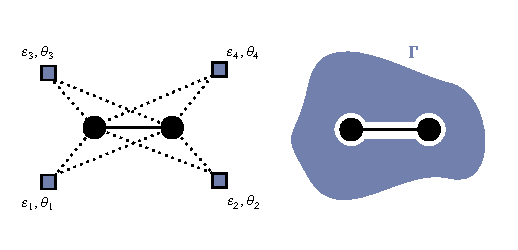
\includegraphics[scale=0.75]{./figures/theory/1D_2s_4b_bulk.pdf}
         \caption{Amas 1D plongé dans un bain sans interactions.}
         \label{fig: amas_CDMFT}
    \end{figure}
\end{frame}

\begin{frame}
    \frametitle{Méthodes numérique - CDMFT}
    \begin{defblock}{Définition: Fonction d'hybridation $\vb{\Gamma}(z)$}
       L'effet du bain sur la fonction de Green est encapsulé dans l'hybridation
        \begin{align}
          \vb{\Gamma}(z) = \Gamma_{ij,\sigma}(z) = \sum_\nu\frac{\theta_{i\nu,\sigma}\theta^*_{j\nu,\sigma}}{z - \epsilon_{\nu,\sigma}},
          \label{eq: hybridization}
        \end{align}
        à l'intérieur de laquelle sont stockés les paramètres variationnels de l'algorithme
        CDMFT.
    \end{defblock}
\end{frame}

\begin{frame}
    \frametitle{Méthodes numérique - CDMFT}
    Grâce au formalisme de base mixte, on calcule la fonction de Green
    \textbf{projetée sur l'amas}
    \begin{align}
        \vb{\Bar{G}}(z) = \Bigg[\frac{N_c}{N}\sum_{\vb{\Tilde{k}}}e^{i\vb{\Tilde{k}}\cdot\vb{\Tilde{r}}}\vb{G}(\vb{\Tilde{k}}, z)\Bigg]_{\vb{\Tilde{r}}=0}
        = \frac{N_c}{N}\sum_{\vb{\tilde{k}}}\frac{1}{z - \vb{t}(\vb{\tilde{k}}) - \textcolor{hard_green}{\vb{\Sigma}_c(z)}}.
    \end{align}
    \pause
    \vfill
    L'essence de la CDMFT est d'obtenir une correspondance entre
    $\vb{G}_c(z)$ et $\vb{\Bar{G}}(z)$ via \textcolor{hard_green}{l'approximation locale de la \textit{self-énergie}:}
    \begin{align}
        \textcolor{hard_green}
        {\vb{\Sigma}(\vb{\tilde{k}}, z)\longrightarrow\vb{\Sigma}_c(z),}
    \end{align}
    dans une boucle d'auto-cohérence.
\end{frame}

\begin{frame}
    \frametitle{Méthodes numériques - CDMFT}
    \begin{columns}
        \column{0.4\linewidth}
        \hspace{1cm}
        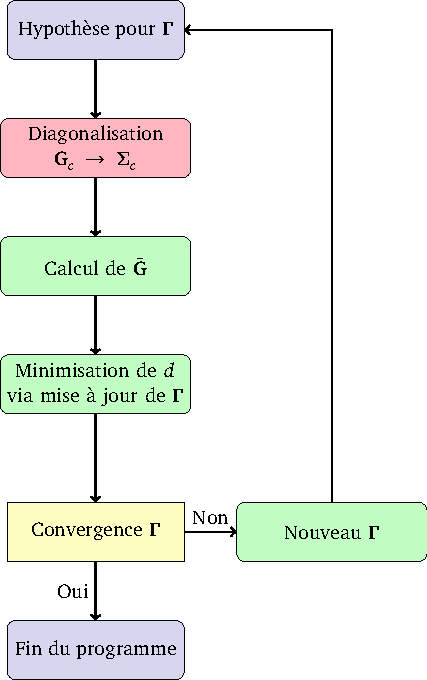
\includegraphics[scale=0.5]{./figures/theory/flow_chart.pdf}
        \column{0.6\linewidth}
        \begin{itemize}
            \item[$\diamond$] Des paramètres $\varepsilon_i, \theta_i$ arbitraires
                sont définit pour l'hybridation d'essai $\vb{\Gamma}(z)$
            \pause
            \item[$\diamond$] Solutionneur d'impureté (ED) pour accéder à
                $\vb{G}_c\to\vb{\Sigma}_c$
            \pause
            \item[$\diamond$] Calcul de la fonction de Green \textbf{projetée sur l'amas} $\vb{\bar{G}}$
            \pause
            \item[$\diamond$] Minimise la fonction de distance $d$ grâce aux paramètres de $\vb{\Gamma}(z)$
            \pause
            \item[$\diamond$] L'hybridation mise à jour est comparée à celle
                de l'itération précédente pour vérifier la convergence
        \end{itemize}
    \end{columns}
\end{frame}

\begin{frame}
    \frametitle{Méthodes numériques - Amélioration de l'auto-cohérence}
    L'idée est de morceler le bain en sous-bains dont un seul est impliqué dans
    la diagonalisation à chaque itération
    \begin{align}
        \vb{\Gamma}(z)\longrightarrow\vb{\Gamma}_1(z) + \vb{\Gamma}_2(z)
    \end{align}
    \begin{figure}
         \centering
         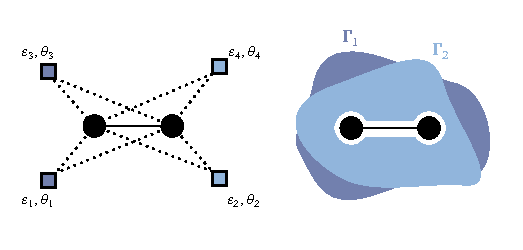
\includegraphics[scale=0.75]{./figures/theory/1D_2s_4vb_bulks.pdf}
         \caption{Amas 1D plongé dans deux sous-bains sans interactions.}
         \label{fig: amas_CDMFT_virtual}
    \end{figure}
\end{frame}

\begin{frame}
    \frametitle{Méthodes numériques - Amélioration de l'auto-cohérence}
    \begin{columns}
        \column{0.25\linewidth}
        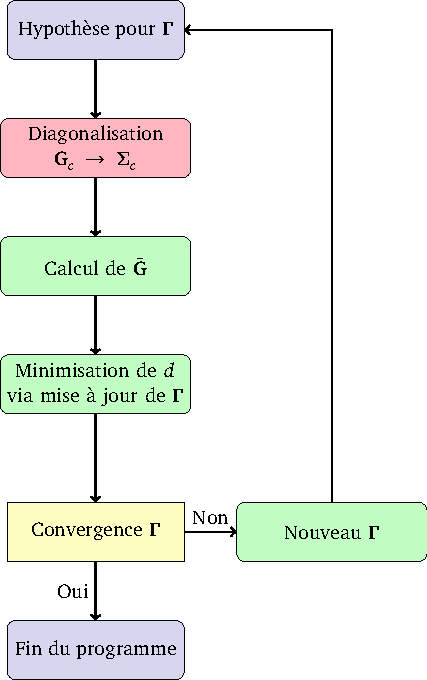
\includegraphics[scale=0.45]{./figures/theory/flow_chart.pdf}
        \column{0.05\linewidth}
        $\longrightarrow$
        \column{0.5\linewidth}
        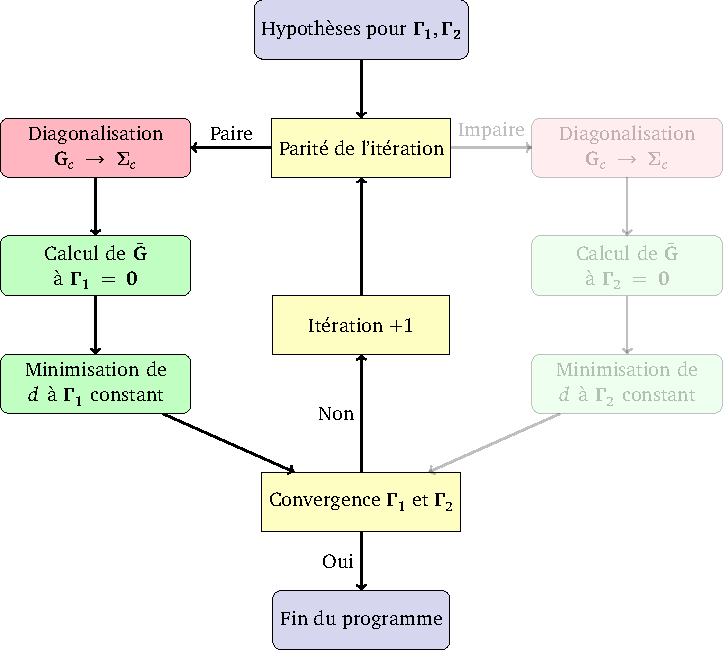
\includegraphics[scale=0.45]{./figures/theory/flow_chart_virtual_pair.pdf}
    \end{columns}
\end{frame}

\begin{frame}
    \frametitle{Méthodes numériques - Amélioration de l'auto-cohérence}
    \begin{columns}
        \column{0.25\linewidth}
        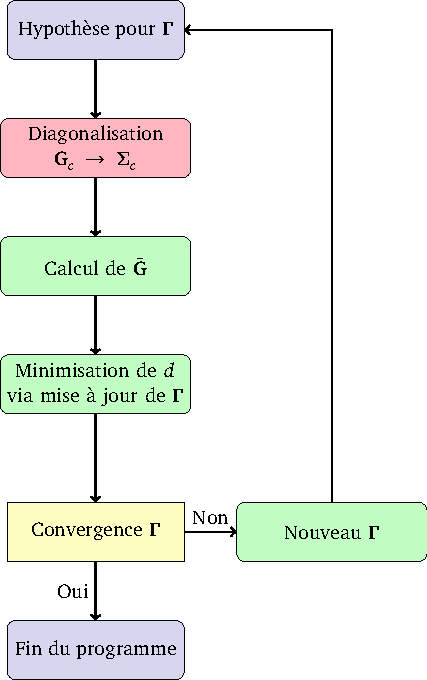
\includegraphics[scale=0.45]{./figures/theory/flow_chart.pdf}
        \column{0.05\linewidth}
        $\longrightarrow$
        \column{0.5\linewidth}
        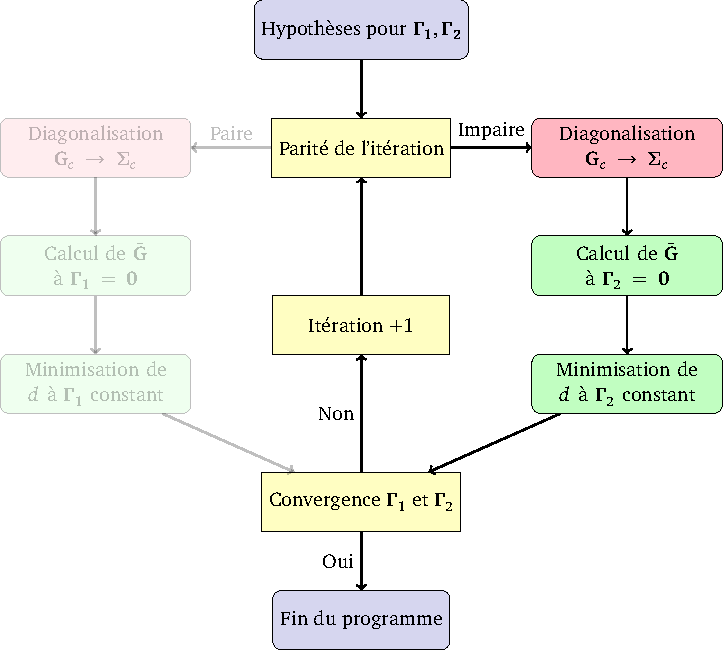
\includegraphics[scale=0.45]{./figures/theory/flow_chart_virtual_impair.pdf}
    \end{columns}
\end{frame}

\begin{frame}
    \frametitle{Méthodes numériques - PyQCM}
        \begin{columns}
            \column{0.5\linewidth}
            {\scriptsize
            \textit{"Pyqcm is a Python/C++ library that implements a few quantum
            cluster methods with an exact diagonalization impurity solver. Quantum
            cluster methods are used in the study of strongly correlated electrons
            to provide an approximate solution to Hubbard-like models\dots"} - David Sénéchal.
            }
            \column{0.5\linewidth}
            \begin{figure}
                 \centering
                 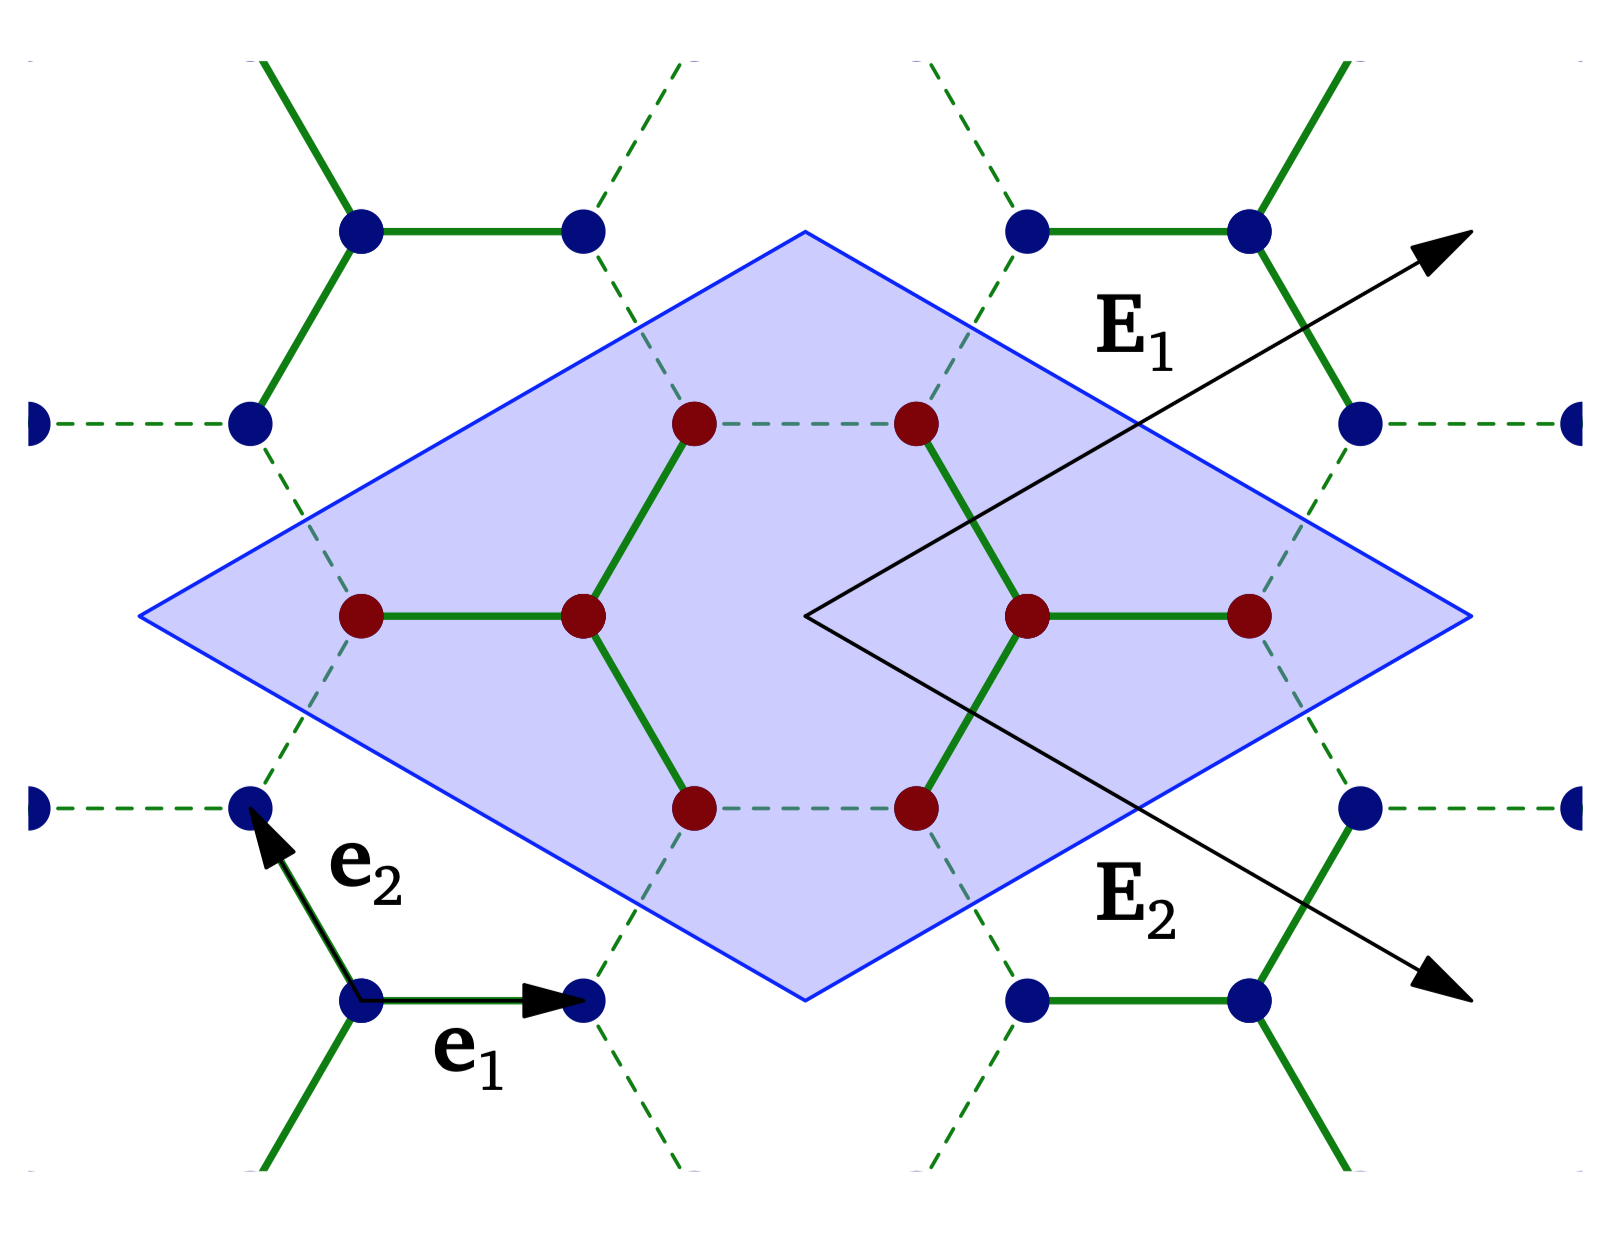
\includegraphics[scale=0.15]{./figures/theory/h8.png}
                 \caption{Réseau cristallin nid d'abeilles\footnotemark.}
                 \label{fig: pyqcm}
            \end{figure}
        \end{columns}
        \footnotetext{\textcolor{refs}{Théo N. DIONNE et al.} Pyqcm: An open-source Python library for quantum cluster methods. \textcolor{sweet_refs}{2023. DOI : 10.21468/SciPostPhysCodeb.23.}}
\end{frame}
